
\subsubsection{Project Description}
%\paragraph{Soft Manipulation}
\hspace*{-10pt}\begin{tabular}{m{11.5cm} m{4cm}}
This work will be carried out within the SoMa project.
SoMa is an project by funded the European Commission Horizon 2020 programme
More details can be found at 
\url{http://www.soma-project.eu}.

This project focusses on the development of {simple, compliant, safe robot manipulation} systems, which are also {robust} and {easy to program}.
It relies on the usage of {soft hands}, that are heavily \textbf{underactuated}.
The compliance of these hands allows them to {adapt} to their environment, while the underactuation significantly simplifies their control, with the price of reduced dexterity.
%The ability to grasp and manipulate objects of different shape, sizes, and materials with soft underactuated hands 
In the proposed approach, the {complex behaviours} required for manipulation are achieved through the exploitation of the physical constraints imposed by the environment.
An example of \textbf{Environmental Constraint Exploitation (ECE)} is shown in Fig.\ref{fig:wall}. The robot pushes the object against a wall, which constrains it and facilitates the grasp.
The project outcomes should be demonstrated in a fruit and vegetable picking scenario and in a context of close \textbf{human-robot physical interaction}.


\subsubsection{Hand Control}
The goal of this project is to develop the \textbf{control primitives} that execute a planned ECE strategy.
The set of behaviours observed in humans for different objects, environments, and perception conditions, must be \textbf{mapped} and transferred to robot systems.
Given an object and a desired grasp strategy, primitives such as approaching, pushing, grasping, etc. are instantiated, sequenced and executed. During execution, \textbf{success} and \textbf{failure} situations must be detected and reported back to the planner.


\subsubsection{Task Overview}
The tasks consist of \textbf{developing a set of controllers} for a robot arm and hand that enables the system to perform \textbf{grasps that exploit environmental constraints}.
These controllers are composed of motion primitives such as \emph{closing the hand}, \emph{pushing against a surface}, \textit{following a trajectory}, etc.
To this end, a cartesian impedance controller on a redundant serial manipulator must be implemented and tuned appropriately to carry out a number of desired behaviours: {\emph{(i)} \textbf{slide} an object along a surface}; \mbox{\emph{(ii)} \textbf{push} and lift an object against a wall};
\mbox{\emph{(iii)} \textbf{flip} an object against one of its edges.}

&
%\begin{figure}
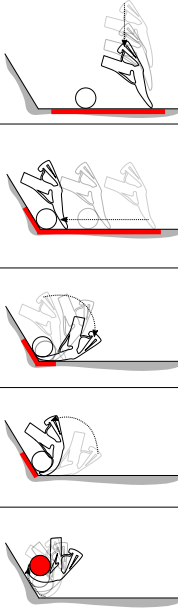
\includegraphics[width=4cm]{figures/wall_grasp}
\captionof{figure}{Wall grasp~\cite{eppner2015exploitation}}\label{fig:wall}
%\end{figure}
\end{tabular}
\subsubsection{Timeline}
\paragraph{Months 1-2}
The student should dedicate the first two months of his project to getting familiar with the hardware and software architecture.
Tutorials and online courses in C++, Python, and ROS (Robot Operating System) programming should be followed, while also learning how to interface with the hardware.
\paragraph{Months 3-4}
During the second part of the project, the student should learn and implement robot motion control strategies and concepts such as inverse kinematics, force and impedance control, as well as online estimation strategies such as Kalman Filters.
The implementation of a prototype controller is done in a simulated environment.
\paragraph{Months 5-6}
In the last part of the project, the developed methods should be implemented on the robot. Performance should be thoroughly tested and a scientific article may be prepared.
\subsubsection{Required Skills}
The successful completion of this project requires that the student possesses or can easily acquire the following skills: 
%\subsection{Technical Skills}
\paragraph{Programming} A significant part of the work will be the development of algorithms and control laws to be executed by the robot. Prototyping is usually done in MATLAB and then implemented in the C++ or Python programming languages.
\paragraph{Linear Algebra} Knowledge of Linear Algebra is essential for developing robot motion control algorithms, particularly  transformations, Jacobian matrices, and matrix operations.
\paragraph{Estimation} Given the uncertainty in the environment and task variability, online estimation of parameters is fundamental to increase the system robustness. The student should be familiar with optimization methods and recursive filtering.

\subsubsection{Outcomes}
The student will become proficient in robot motion \textbf{control}. He will learn advanced concepts of robot kinematics and dynamics.
Furthermore, he will have the experience of working in a \textbf{research} environment, obtaining \textbf{experimental} skills, the ability to work independently and in a group. He will also learn how to do data analysis, scientific writing, systems engineering and programming.
The results of the student project will be included in the final demonstrator to be presented to project reviewers.